\documentclass[12pt]{article}
\usepackage[T2A]{fontenc}
\usepackage[utf8]{inputenc}
\usepackage[russian]{babel}
\usepackage{amsmath, graphicx, float, hyperref}

\begin{document}
    \begin{titlepage}
        \begin{center}
            \vspace*{1cm}

            \Huge
            \textbf{Закон всемирного тяготения.\\Точки Лагранжа}

            \vspace{1.5cm}

            \Large
            \textbf{Балдин Виктор Б01-303}

            \vfill

            Вопрос по выбору \\
            Устный экзамен по общей физике

            \vspace{0.8cm}

            
\includegraphics[width=0.4\textwidth]{university_logo.png}

            Физтех-школа радиотехники и компьютерных технологий\\
            Московский физико-технический институт\\
            Долгопрудный, 2024
        \end{center}
    \end{titlepage}

    \begin{abstract}
        \par Данный вопрос по выбору включает в себя теоретические расчеты
        положения точек Лагранжа и обсуждение некоторых их интересных
        свойств. В работе используются материалы из различных открытых
        источников об истории исследований на эту тему и современном их
        состоянии.
        \par Точки Лагранжа являются крайне важным объектом для изучения
        космического пространства в современной астрофизике.
        В частности, прямым образом их свойства используются для размещения
        космических аппаратов, предназначенных для наблюдений дальнего
        космоса.
        \par Автор выражает надежду, что данная работа содержит
        актуальные сведения и благодарит экзаменационную комиссию за ее
        рассмотрение.
    \end{abstract}

    \newpage

    \section{Введение}
    \par \textit{Точки Лагранжа}, в некоторых источниках также \textit{точки
    либрации} или \textit{$L$-точки} -- точки в системе двух тел, в которых
    третье тело может оставаться неподвижным относительно первых двух.
    \par Нахождение точек Лагранжа является частным случаем решения задачи
    трех тел для случая круговых орбит и малой массы одного из них. То есть,
    другими словами, два массивных тела равномерно вращаются вокруг общего
    центра масс. В этой ситуации существует 5 точек, в которых третье
    невесомое (обладающее пренебрежимо малой массой) тело может оставаться
    неподвижным в системе отсчета, связанной с массивными телами.
    \par Точки Лагранжа названы в честь математика Жозефа Луи Лагранжа,
    который первым в 1772 году показал их существование.
    \begin{figure}[H]
        \centering
        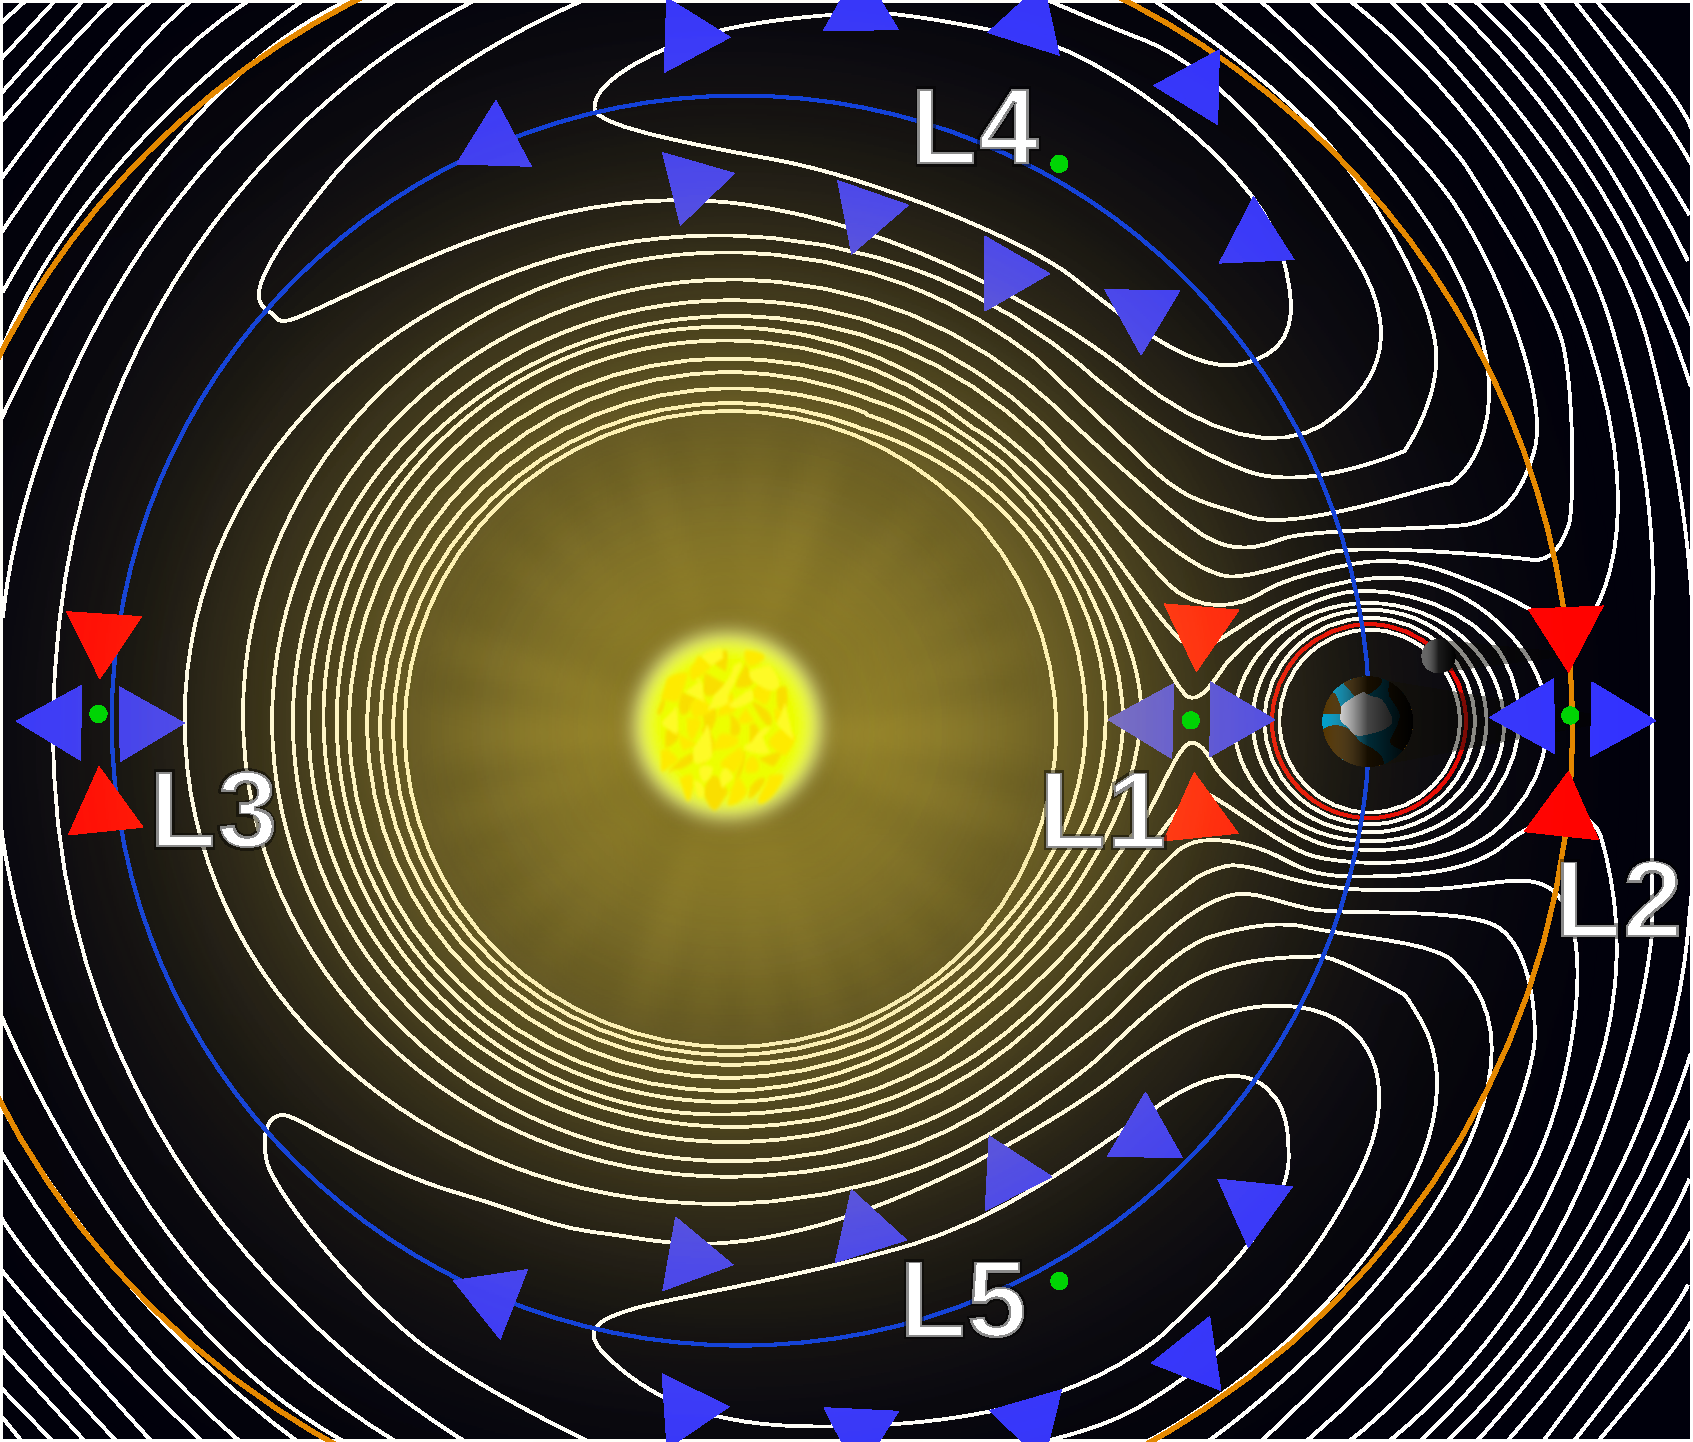
\includegraphics[scale=0.35]{Lagrange_points.pdf}
        \caption{5 точек Лагранжа и гравитационные эквипотенциальные
        поверхности системы двух тел\\
        \textit{Источник:}
        \url{https://upload.wikimedia.org/wikipedia/commons/thumb/e/ee/
        Lagrange_points2.svg/1920px-Lagrange_points2.svg.png}}
    \end{figure}

    \section{Задача 3-х тел}
    Для начала проведем краткое рассмотрение движения 3-х тел, связанных между
    собой гравитационными взаимодействиями. Это может быть описано в общем
    случае следующими дифференциальными уравнениями:
    \begin{equation}
        \begin{cases}
            \ddot{\vec{r_1}} = -Gm_2\frac{\vec{r_1} - \vec{r_2}}
            {\lvert \vec{r_1} - \vec{r_2} \rvert} -
            Gm_3\frac{\vec{r_1} - \vec{r_3}}{\lvert \vec{r_1} - 
            \vec{r_3} \rvert}\\
            \ddot{\vec{r_2}} = -Gm_2\frac{\vec{r_2} - \vec{r_3}}
            {\lvert \vec{r_2} - \vec{r_3} \rvert} -
            Gm_3\frac{\vec{r_2} - \vec{r_1}}{\lvert \vec{r_2} - 
            \vec{r_1} \rvert}\\
            \ddot{\vec{r_3}} = -Gm_2\frac{\vec{r_3} - \vec{r_1}}
            {\lvert \vec{r_3} - \vec{r_1} \rvert} -
            Gm_3\frac{\vec{r_3} - \vec{r_2}}{\lvert \vec{r_3} - 
            \vec{r_2} \rvert}\\
        \end{cases}\,.
    \end{equation}

    \section{Вычисление точек Лагранжа}
    Все точки Лагранжа находятся в плоскости орбит массивных тел. Их можно
    разбить на 2 подвида:
    \begin{enumerate}
        \item \textit{Коллинеарные} ($L_1$, $L_2$, $L_3$) -- расположены на прямой,
        соединяющей 2 массивных тела.
        \item \textit{Треугольные} или \textit{троянские} ($L_4$, $L_5$).
    \end{enumerate}
    \par Введем следующие обозначения: $M_1$, $M_2$ -- массы массивных тел,
    $m$ -- масса малого тела, при этом $m \ll M_1, M_2$, $R$ -- расстояние
    между телами.
    \par Удобно найти расстояние до центра масс от каждого из тел. По
    определению центра масс
    $$ M_2(R - r_1) - M_1r_1 = 0, $$
    откуда
    $$ r_1 = \frac{M_2}{M_1 + M_2}R $$
    Введя обозначение
    $$ \alpha = \frac{M_2}{M_1 + M_2}, $$
    получим $r_1 = \alpha R$, $r_2 = (\alpha - 1)R$.
    Введем систему координат с началом координат в центре масс системы
    и осью, направленной от $M_1$ к $M_2$.

    \subsection{Коллинеарные точки Лагранжа}
    \par $L_1$ -- точка, находящаяся между двумя массивными телами. Запишем для
    массы $m$ в этой точке второй закон Ньютона:

    \begin{equation}
        \frac{GM_1m}{(L_1 - r_1)^2} - \frac{GM_2m}{(L_1 - r_2)^2} = m\Omega^2r
        \label{L1}
    \end{equation}

    \par Найдем угловую скорость вращения тел из третьего закона Кеплера:

    \begin{equation}
        \Omega^2 = \frac{G(M_1 + M_2)}{R^3}
        \label{kepler}
    \end{equation}

    Комбинируя \ref{L1} и \ref{kepler} несложно свести это к
    следующему уравнению:

    \begin{equation}
        \frac{M_1}{(L_1 - r_1)^2} - \frac{M_2}{(L_1 - r_2)^2} =
        r\frac{M_1 + M_2}{R^3}
        \label{eq1}
    \end{equation}

    Как нетрудно видеть, это сводится к уравнению 5-й степени относительно $r$,
    что делает невозможным его общее алгебраическое решение. Поэтому получить
    формулу мы можем лишь приближенно для значений $\alpha \ll 1$, то есть для
    случая, когда масса $m \ll M_2 \ll M_1$.
    \par В этом случае решение уравнения \ref{eq1} принимает вид

    \begin{equation}
        L_1 = R\left(1 - \left(\frac{\alpha}{3}\right)^{1/3}\right)
    \end{equation}

    \par Хорошим примером системы, удовлетворяющей соотношению $\alpha \ll 1$,
    является система Земля -- Солнце. В самом деле,
    $\alpha \approx 3 \cdot 10^{-6}$, $R = 1{,}5 \cdot 10^8$ км.
    $L_1$ для этой системы лежит на расстоянии $R - L_1 \approx 1{,}5 \cdot 10^6$
    км от Земли.

    \par Очень схожим образом находится $L_2$ -- точка Лагранжа, расположенная
    за менее массивным телом ($M_2$). Для нее при $\alpha \ll 1$ примерное
    решение

    \begin{equation}
        L_2 = R\left(1 + \left(\frac{\alpha}{3}\right)^{1/3}\right)
    \end{equation}

    \par Как можно видеть, $L_1$ и $L_2$ в этом случае симметричны относительно
    наименее массивного тела $M_2$.

    Несколько другой результат мы получим для точки $L_3$:

    \begin{equation}
        L_3 = -R\left(1 + \frac{5}{12}\alpha\right)
    \end{equation}

    \begin{thebibliography}{10}
        \bibitem{enwikipedia}
        \url{https://en.wikipedia.org/wiki/Lagrange_point}

        \bibitem{mit18}
        \url{https://ocw.mit.edu/courses/16-07-dynamics-fall-2009/resources/mit16_07f09_lec18/}

        \bibitem{nasa}
        \url{https://wmap.gsfc.nasa.gov/media/ContentMedia/lagrange.pdf}
    \end{thebibliography}

\end{document}
